% this file is called up by thesis.tex
% content in this file will be fed into the main document

%: ----------------------- name of chapter  -------------------------
\chapter{Mô hình hệ thống theo dõi tin tức trực tuyến $\mathcal{N}$\texttt{ewSOMoni}} % top level followed by section, subsection


%: ----------------------- paths to graphics ------------------------

% change according to folder and file names
\ifpdf
    \graphicspath{{3/figures/PNG/}{3/figures/PDF/}{3/figures/}}
\else
    \graphicspath{{3/figures/EPS/}{3/figures/}}
\fi

%: ----------------------- contents from here ------------------------


\noindent Chương này chúng tôi sẽ trình bày về hệ thống theo dõi tin tức trực tuyến có tên $\mathcal{N}$\texttt{ewSOMoni}
\footnote{[nju: 's$\Lambda$m m$\Lambda$ni]} \footnote{$\mathcal{N}$\texttt{ew} \overbrace{S}^{\mbox{Smartness}} \underbrace{O}_{\mbox{Orientation}} \overbrace{M}^{\mbox{Magnitude}}oni \hspace{0.2in}   \mbox{viết tắt của \texttt{News Online Monitoring}}} cùng  phương pháp lai giữa luật và học máy Maximum Entropy để  trích xuất sự kiện.
%Trước tiên, mô hình đề xuất và diễn giải chi tiết hệ thống được thể hiện ở phần %\ref{system} ngay dưới đây. Sau đó, phương pháp lai trích xuất sự kiện được nói %tới  ở phần \ref{method} (trang \pageref{method}).
%Trước tiên, phương pháp lai giữa luật ngữ nghĩa và học máy Maximum Entropy được 
Trước tiên, phương pháp  đánh giá hiệu quả trích xuất sẽ được nói tới nhằm mục đích làm rõ tiêu chí ước lượng phương pháp trích xuất và làm cơ sở để so sánh phương pháp của chúng tôi với các  phương pháp khác. Tiếp sau, mô hình đề xuất và diễn giải chi tiết của hệ thống $\mathcal{N}$\texttt{ewSOMoni} được xem xét ở phần \ref{system}.
%Trước tiên, phương pháp đánh giá hệ thống được


%\section{Kết hợp luật ngữ nghĩa  và Maximum Entropy trong trích xuất sự kiện}
%\label{method}
\section{Phương pháp đánh giá hiệu quả trích xuất sự kiện}
\noindent Mọi phương pháp trích xuất sự kiện được đề xuất đều phải đánh giá hiệu quả trích xuất. Tuy vậy, để đánh giá hiệu quả trích xuất một cách tự động là công việc khó vì tính bất định của sự kiện hàng ngày.
%Điều đó có nghĩa rằng luôn cần có sự can thiệp của con người trong quá trình %ánh giá.
Hội nghị MUC định nghĩa các khung mẫu sự kiện với các trường chưa được xác định. Công việc của các nhà nghiên cứu là tìm cách xác định những trường này. Bởi thế, ước lượng phương pháp trích xuất sự kiện sử dụng độ chính xác và độ hồi tưởng được tính bởi các công thức \ref{eq:precision}, \ref{eq:recall} \cite{RB96}.

\begin{equation}
  \label{eq:precision}
  \mbox{độ chính xác} = \frac{N_{\mbox{điền đúng}}}{N_{\mbox{điền đúng}} + N_{\mbox{điền sai}}}
\end{equation}


\begin{equation}
  \label{eq:recall}
  \mbox{độ hồi tưởng} = \frac{N_{\mbox{điền đúng}}}{N_{\mbox{phải điền}}}
\end{equation}
\noindent Trong đó:
\begin{itemize}
  \item $N_{\mbox{phải điền}}$ \hspace{0.5cm}là số trường trong khung mẫu phải điền vào
  \item $N_{\mbox{điền đúng}}$ \hspace{0.5cm} là số trường mà phương pháp điền được và  đúng
    \item $N_{\mbox{điền sai}}$ \hspace{0.5cm} là số trường mà phương pháp điền được nhưng sai
\end{itemize}

\noindent Chương trình ACE,






\section{Hệ thống theo dõi tin tức trực tuyến  $\mathcal{N}$\texttt{ewSOMoni}}
\label{system}
%\figuremacro{largepotato}{Mô hình hệ thống}{ok}}
%\figuremacro{system}{Mô hình hệ thống}}
\noindent Công trình nghiên cứu này chúng tôi đã xây dựng một hệ thống theo dõi tin tức trực tuyến. Nhiệm vụ chính của hệ thống là quan sát tức mới được đưa lên các nguồn cung cấp tin tức (phụ lục \ref{website}, trang \pageref{website}), phân loại và nhận dạng  sự kiện thuộc ba lĩnh vực: \textsc{Tai nạn giao thông}, \textsc{Hình sự}, \textsc{Cháy nổ}. Cuối cùng là trực quan hóa trên bản đồ cho người dùng dễ dàng theo dõi, cập nhật. \\
\noindent Mô hình của hệ thống được thể hiện rõ ở hình \ref{fig:system}. Hệ thống $\mathcal{N}$\texttt{ewSOMoni} có năm  phần chính:
\begin{figure}[htbp]
		\centering
		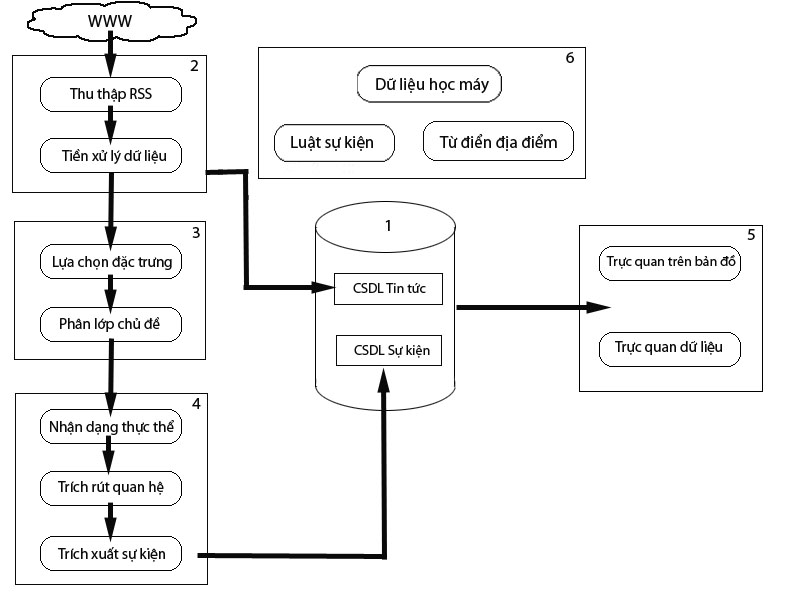
\includegraphics[width=1\textwidth]{system}
		\caption{\textbf{Mô hình hệ thống  $\mathcal{N}$\texttt{ewSOMoni}}}
		\label{fig:system}
\end{figure}

\begin{itemize}
  \item \textbf{Kho dữ liệu} cơ sở dữ không ràng buộc, hướng tài liệu (MongoDB), lưu trữ lượng  lớn dữ liệu tin tức

\item \textbf{Thu thập dữ liệu} thu thập dữ liệu tự động và tiền xử lý dữ liệu
  \item \textbf{Phân lớp chủ đề} đưa  tin tức thu thập được vào hai  dạng: \textsc{Sự kiện}, \textsc{Không phải sự kiện}

    %\textsc{Tai nạn giao thông}, \textsc{Hình sự}, \textsc{Cháy nổ}, %\textsc{Còn lại}.


  \item \textbf{Trích xuất sự kiện} thực hiện các bước cần thiết để trích xuất sự kiện
  \item \textbf{Trực quan hóa dữ liệu} có nhiệm vụ tương tác với cơ sở dữ liệu để hiển thị thông tin cho người dùng
 \end{itemize}

\noindent Mỗi thành phần của hệ thống sẽ được diễn giải chi tiết dưới đây.

\subsection{Kho dữ liệu}
\label{db}
\noindent Hệ thống phải xử lý dữ liệu lớn nên cần lựa chọn kiểu lưu trữ cũng như thiết kế cơ sở dữ liệu phù hợp. Riêng chỉ lượng dữ liệu thu thập ngoại tuyến gồm 3.842.137 tin tức điện tử phục vụ cho quá trình sinh luật và học mô hình phân lớp ban đầu đã có dung lượng gần 60GB. Hơn nữa, hệ thống chạy trực tuyến mỗi ngày nhận khoảng 1500 bài báo điện tử. Do vậy, cần thiết một hệ cơ sở dữ liệu có khả năng truy xuất dữ liệu nhanh cũng như có khả năng mở rộng về sau. Qua khảo sát, nhóm nghiên cứu nhận thấy các hệ cơ sở dữ liệu không quan hệ (NoSQL) phù hợp với tiêu chí đề ra. NoSQL không tồn tại các ràng buộc giữa các bảng lưu trữ. Điều này giúp cho tốc độ truy vấn tốt hơn hẳn so với các hệ cơ sở dữ liệu quan hệ truyền thống. Thứ nữa, NoSQL là hệ cơ sở dữ liệu phân tán, có thể mở rộng theo chiều ngang, nghĩa là các yếu tố phần cứng như bộ nhớ ngoài (HDD), bộ nhớ trong (RAM) có thể tăng thêm bằng cách kết hợp nhiều thành phần phần cứng nhỏ hơn với nhau. Với khoảng 15 năm phát triển \footnote{NoSQL lần đầu tiên được giới thiệu vào năm 1998 bởi Carlo Strozzi}, đã có rất nhiều hệ cơ sở dữ liệu thuộc họ NoSQL ra đời. Ví dụ, lưu trữ dạng tài liệu có MongoDB, CouchDB, BaseX; lưu trữ dạng đồ thị có Neo4j, OrientDB, Sones GraphDB; lưu trữ dạng key--value có BigTable, Cassandra, Redis \footnote{\href{http://http://en.wikipedia.org/wiki/NoSQL}{http://en.wikipedia.org/wiki/NoSQL}}. BigTable được Google \footnote{\href{www.google.com}{www.google.com}} sử dụng, Cassandra là sản phẩm của mạng xã hội Facebook \footnote{\href{http://www.facebook.com/}{http://www.facebook.com/}}, mạng xã hội của giới lập trình viên Github \footnote{\href{http://github.com/}{https://github.com/}} sử dụng Redis, MongoDB được dùng bởi mạng xã hội Foursquare \footnote{\href{http://foursquare.com/}{http://foursquare.com/}} là những cái tên nổi bật hơn cả.  Trong nghiên cứu này, chúng tôi lựa chọn hệ cơ sở dữ liệu MongoDB làm thành phần lưu trữ dữ liệu bởi khả năng truy vấn dữ liệu nhanh, tự động dàn trải dữ liệu và dễ dàng phân tán.
\\
\noindent Kho dữ liệu gồm hai phần: cơ sở dữ liệu tin tức, cơ sở dữ liệu sự kiện.
\paragraph{Cơ sở dữ liệu tin tức} $\;$ \\
\emph{Đầu vào:} tin tức từ bộ thu thập dữ liệu sau khi đã tiền xử lý dữ liệu (Pha 2).

\paragraph{Cơ sở dữ liệu sự kiện} $\;$ \\
\emph{Đầu vào:} sự kiện và các thông tin về sự kiện đó từ pha trích xuất sự kiện (Pha 4).


\subsection{Thu thập dữ liệu}
\label{datacrawler}
\noindent Hiện nay, hầu hết các trang tin tức đều cung cấp cơ chế chia sẻ tin RSS. Tận dụng tính năng này, một bộ thu thập dữ liệu qua RSS được xây dựng.

\paragraph{Thu thập tin tức RSS} $\;$\\
\noindent Tin tức từ các kênh RSS của các trang tin tức điện tử theo dạng XML như hình \ref{fig:xml} được tự động thu thập qua bộ RSSFeeder.

\begin{figure}[htbp]
		\centering
		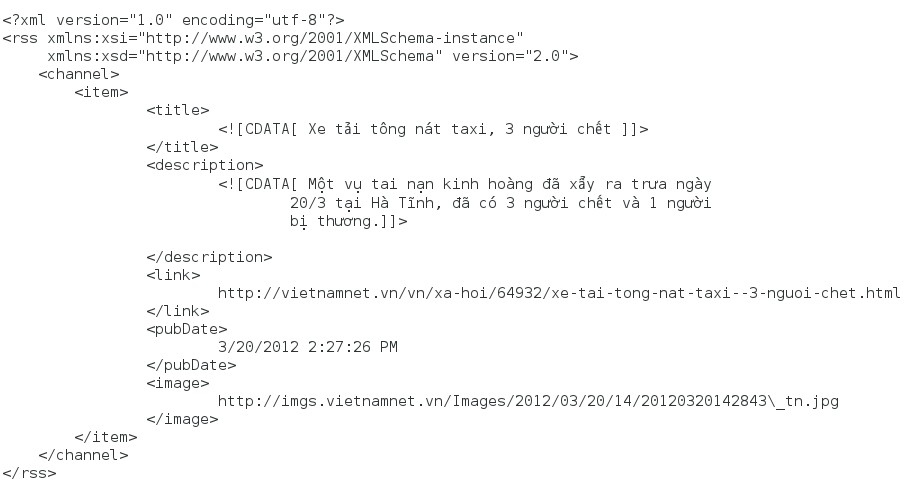
\includegraphics[width=1\textwidth, height=3.5in]{xmlformat}
		\caption{\textbf{Khuôn dạng tin tức lấy qua kênh RSS}}
		\label{fig:xml}
\end{figure}


\paragraph{Tiền xử lý dữ liệu} $\;$ \\
\noindent Sau khi bộ RSSFeeder lấy tin tức về, dữ liệu cần phải lọc ra những thông tin cần thiết. Hai lý do cần thiết để làm việc này. Một là giảm dung lượng dữ liệu lưu trữ trên hệ thống. Hai là giúp cho các bước xử lý sau dễ dàng hơn. \\
\noindent \emph{Đầu vào} là các bản tin có định dạng như hình \ref{fig:xml} \\
\noindent \emph{Đầu ra} là các thông tin bao gồm: tiêu đề, tóm tắt, đường dẫn tới bài báo và ngày đăng tin. Bảng \ref{tb:rawdata} là một ví dụ cho nội dung tin tức thể hiện ở hình \ref{fig:xml}. Dữ liệu sau khi tiền xử lý được lưu trữ trong  cơ sở dữ liệu tin tức. \\

\begin{table}
	\centering
\caption{\textbf{Dữ liệu sau khi tiền xử lý} }
  \begin{tabular}{|l|l|}
     \hline
     \textbf{Tên trường} & \textbf{Giá trị} \\
     \hline
     Tiêu đề & Xe tải tông nát taxi, 3 người chết \\
     \hline
     Tóm tắt & Một vụ tai nạn kinh hoàng đã xẩy ra trưa ngày 20/3 \\
     $\;$ $\;$ $\;$ $\;$ $\;$ $\;$ $\;$ $\;$ &	tại Hà Tĩnh, đã có 3 người chết và 1 người bị thương. \\
     \hline
     Đường dẫn & vietnamnet.vn/vn/xa-hoi/64932/xe-tai-tong-nat-taxi--3-nguoi-chet.html \\
     \hline
     Ngày đăng tin & 3/20/2012 2:27:26 PM \\
     \hline
  \end{tabular}

  \label{tb:rawdata}
\end{table}



\subsection{Phân loại sự kiện}
\label{classifi}

\noindent Pha này sẽ giải quyết vấn đề nhận dạng sự kiện. Tin tức thu được từ pha  thu thập dữ liệu sẽ được quyết định có chứa sự kiện hay không. Qua khảo sát dữ liệu, chúng tôi nhận thấy hầu hết tiêu đề tin tức thể hiện rõ được nội dung tin tức có nói về sự kiện. Bởi vậy, bài toán đưa về phân lớp nhị phân mức câu. Đây là bước đầu tiên trong quá trình kết hợp luật ngữ nghĩa và học máy để trích xuất sự kiện mà chung tôi đề xuất. Hai việc cần phải làm trong pha này. Đầu tiên, tập đặc trưng được lựa chọn. Các đặc trưng sẽ được trích chọn trên tập tin tức đã thu thập trước (dữ liệu ngoại tuyến). Sau đó, mô hình phân lớp được sinh ra bằng  phương pháp học máy Maximum Entropy. Tin tức qua mô hình phân lớp hoặc được truyền tới pha tiếp theo nếu được nhận dạng là chứa sự kiện, hoặc bị loại bỏ nếu ngược lại.

\paragraph{Lựa chọn và trích chọn đặc trưng}  $\;$ \\


\paragraph{Phân lớp chủ đề} $\;$ \\
%\noindent



\subsection{Trích xuất sự kiện}
\label{ee}
\noindent Sau khi đã nhận dạng được tin tức có chứa sự kiện, sự kiện cùng ba thông tin liên quan: người, thời gian, địa điểm sẽ được trích xuất. Ba vấn đề cần giải quyết để hoàn thành pha này gồm có trích chọn thực thể, trích xuất quan hệ thực thể và trích xuất sự kiện. Hai vấn đề đầu tiên chúng tôi sử dụng kết quả kế thừa từ các nghiên cứu XYZ, TUV  của phòng thí nghiệm Công Nghệ Tri Thức (KT--Lab). Giải quyết vấn đề thứ ba là bước thứ hai và cũng là bước cuối cùng trong quá trình kết hợp luật ngữ nghĩa và học máy Maximum Entropy để trích xuất sự kiện. \\



\paragraph{Trích chọn thực thể}



\paragraph{Trích xuất quan hệ thực thể}


\paragraph{Trích xuất sự kiện}
\noindent


\subsection{Trực quan hóa dữ liệu}
\label{vi}
\noindent Pha trực quan hóa dữ liệu lấy sự kiện cùng các thông tin liên quan và thể hiện trực quan trên bản đồ do Google Map \footnote{\href{https://developers.google.com/maps/}{https://developers.google.com/maps/}} cung cấp.


%Insert ảnh màn hình  vào đây.





% ---------------------------------------------------------------------------
%: ----------------------- end of thesis sub-document ------------------------
% ---------------------------------------------------------------------------
